\clearpage
\subsection{Prompts and Generation Settings}
The following templates come from the paired-prediction collection. Number words for 4 and 16 are displayed as digits here. The original prompt files are retained with the code. Placeholders are replaced by each sample's expression or statement. CUB supplies all 200 candidate classes in a single request; its full class list is supplied with the code. Both VLMs receive the same task input, but their templates may differ. All requests use temperature zero, with limits of 8 tokens for CUB and NLVR2, 512 for gRefCOCO and 768 for ConstructionSite. NLVR2 sends the left image followed by the right image, with these roles explicitly marked. Qwen disables thinking for CUB and NLVR2; MiniCPM constrains these answers to the class index or True/False. Localization and event requests use JSON schemas. Invalid answers are retained and counted as errors without repair or a second model call.

\subsubsection{CUB-200-2011}
\paragraph{MiniCPM-V-4.5}
\VerbatimInput[fontsize=\footnotesize,breaklines=true,breakanywhere=true]{data/reproduction/cub_MiniCPM_prompt.txt}
\paragraph{Qwen3.8-27B-FP8}
\VerbatimInput[fontsize=\footnotesize,breaklines=true,breakanywhere=true]{data/reproduction/cub_Qwen3.8_prompt.txt}

\subsubsection{gRefCOCO}
\paragraph{MiniCPM-V-4.5}
\VerbatimInput[fontsize=\footnotesize,breaklines=true,breakanywhere=true]{data/reproduction/grefcoco_MiniCPM_display.txt}
\paragraph{Qwen3.8-27B-FP8}
\VerbatimInput[fontsize=\footnotesize,breaklines=true,breakanywhere=true]{data/reproduction/grefcoco_Qwen3.8_prompt.txt}

\subsubsection{NLVR2}
\paragraph{MiniCPM-V-4.5}
\VerbatimInput[fontsize=\footnotesize,breaklines=true,breakanywhere=true]{data/reproduction/nlvr2_MiniCPM_prompt.txt}
\paragraph{Qwen3.8-27B-FP8}
\VerbatimInput[fontsize=\footnotesize,breaklines=true,breakanywhere=true]{data/reproduction/nlvr2_Qwen3.8_prompt.txt}

\subsubsection{ConstructionSite}
\paragraph{MiniCPM-V-4.5}
\VerbatimInput[fontsize=\footnotesize,breaklines=true,breakanywhere=true]{data/reproduction/construction_MiniCPM_display.txt}
\paragraph{Qwen3.8-27B-FP8}
\VerbatimInput[fontsize=\footnotesize,breaklines=true,breakanywhere=true]{data/reproduction/construction_Qwen3.8_display.txt}

\clearpage
\subsection{Earlier Prompt Comparisons}
Figures below reproduce earlier prompt comparisons on training subsets: 300 expressions for gRefCOCO and 400 examples each for CUB and NLVR2. Construction uses its recorded training selection. The source label Construction10K refers to ConstructionSite. These curves use the earlier task metrics (including gRefCOCO F1), so their absolute values are not directly comparable with the final routing table. They document prompt choice, not router ablations or new test-time tuning. The experiment ledger retains the input subset and metric for every point.
\begin{figure}[H]\centering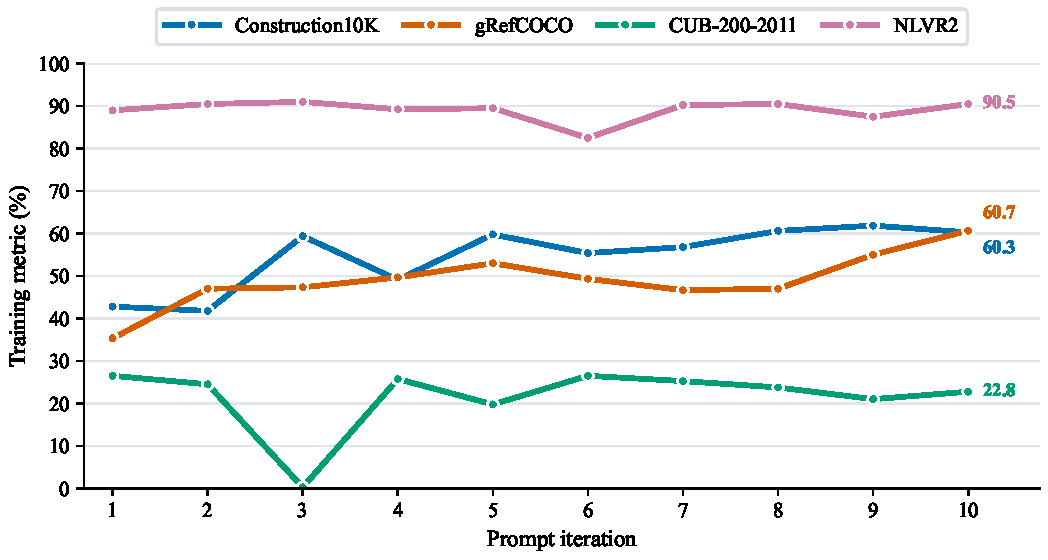
\includegraphics[width=\textwidth]{figures/prompt_iteration_curves_minicpm.pdf}\caption{Earlier MiniCPM prompt comparisons from the recorded experiment ledger.}\end{figure}
\begin{figure}[H]\centering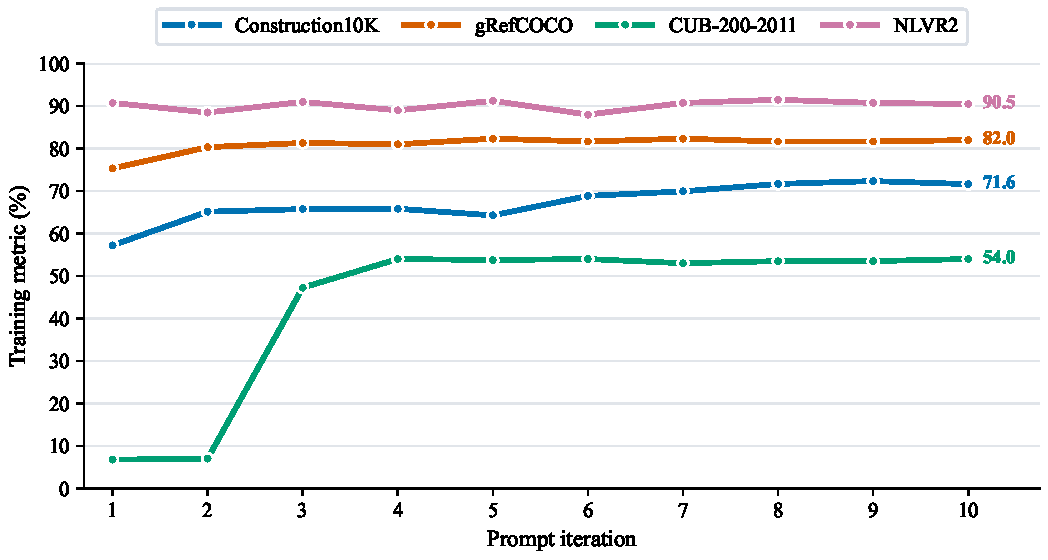
\includegraphics[width=\textwidth]{figures/prompt_iteration_curves_qwen38.pdf}\caption{Earlier Qwen prompt comparisons from the same ledger.}\end{figure}
